\documentclass[12pt]{article}

\setlength{\parindent}{0em}
\setlength{\parskip}{.5em}

\usepackage{framed}
\newcounter{problem}
\newcounter{problempart}[problem]
\newcounter{solutionpart}[problem]
\newenvironment{problem}{\stepcounter{problem}\noindent{\bf\arabic{problem}.}}{\setcounter{problempart}{0}\setcounter{solutionpart}{0}}
\newenvironment{solution}{\par\textcolor{blue}\bgroup}{\egroup\par}
\newcommand{\qpart}{\stepcounter{problempart}${}$\\\noindent{(\alph{problempart})} }
\newcommand{\spart}{\stepcounter{solutionpart}${}$\\\noindent{(\alph{solutionpart})} }
\newcommand{\TODO}{\textcolor{red}{$\blacksquare$}}
\newcommand{\SOL}[1]{\textcolor{blue}{#1}}

\usepackage{hyperref}
\usepackage{fullpage}
\usepackage{amsmath,mathabx,MnSymbol}
\usepackage{color,tikz}
\usepackage{footnote,enumitem}
\usepackage{longtable}
\newcommand{\mx}[1]{\begin{pmatrix}#1\end{pmatrix}}
\definecolor{dkgreen}{rgb}{0,.5,0}
\usepackage{algorithm}
\usepackage[noend]{algpseudocode}

\newcommand{\uu}{\mathbf{u}}
\newcommand{\vv}{\mathbf{v}}
\newcommand{\cc}{\mathbf{c}}
\newcommand{\ww}{\mathbf{w}}
\newcommand{\xx}{\mathbf{x}}
\newcommand{\zz}{\mathbf{z}}
\newcommand{\ee}{\mathbf{e}}
\newcommand{\pp}{\mathbf{p}}
\newcommand{\qq}{\mathbf{q}}
\renewcommand{\AA}{\mathbf{A}}
\newcommand{\BB}{\mathbf{B}}
\newcommand{\CC}{\mathbf{C}}
\newcommand{\DD}{\mathbf{D}}
\newcommand{\nn}{\mathbf{n}}
\newcommand{\gp}[1]{\left(#1\right)}

\newcommand{\TODOL}[1]{\textcolor{red}{\underline{\hspace{#1 cm}}}}

\usepackage{listings}

\lstset{
  language=C++,
  showstringspaces=false,
  identifierstyle=\color{magenta},
  basicstyle=\color{magenta},
  keywordstyle=\color{blue},
  identifierstyle=\color{black},
  commentstyle=\color{green},
  stringstyle=\color{red}
}

\begin{document}

\title{CS130 - Math review}
\date{}
\author{Name: \TODOL7\qquad\qquad SID: \TODOL4}
\maketitle
\begin{center}
\end{center}

\section*{Part 1: vectors, dot and cross product}

\begin{problem}
Calculate the cosine of the angle between the vectors $\mx{2\\ 4\\ 4}$ and
$\mx{4\\ 3\\ 0}$.
\end{problem}

\begin{solution}
  \textbf{\textcolor{red}{\TODO}}
\end{solution}

\begin{problem}
Consider a plane containing the point $P = (1,3,-1)$, with normal $\nn = (\frac{1}{3},\frac{2}{3},-\frac{2}{3})$.
Let $Q = (5,6,7)$ be a point (not on the plane).  For each point below, indicate whether the point is on the plane, on the same side of the plane as $Q$, or on the opposite side of the plane from $Q$.
\begin{enumerate}
\item $(0,0,0)$
\item $(-1,1,2)$
\item $(1,4,0)$
\item $(1,5,1)$
\item $(-1,-1,-1)$
\end{enumerate}
\end{problem}

\begin{solution}
  \textbf{\textcolor{red}{\TODO}}
\end{solution}

\begin{problem}
Calculate the cross product: $\mx{1\\ 2\\ 3} \times \mx{4\\ 5\\ 6}$.
\end{problem}

\begin{solution}
  \textbf{\textcolor{red}{\TODO}}
\end{solution}

\begin{problem}
Calculate a vector $\ww$ in the same direction of the vector $\uu$ and that has
the same length as the vector $\vv$.
\end{problem}

\begin{solution}
  \textbf{\textcolor{red}{\TODO}}
\end{solution}

\begin{problem}
  Consider a triangle with sides $\uu$ (of length $a$), $\vv$ (of length $b$), and $\uu - \vv$ (of length $c$), with the angle between $\uu$ and $\vv$ equal to $\theta$ as shown in the two figures below.\\
\begin{center}
  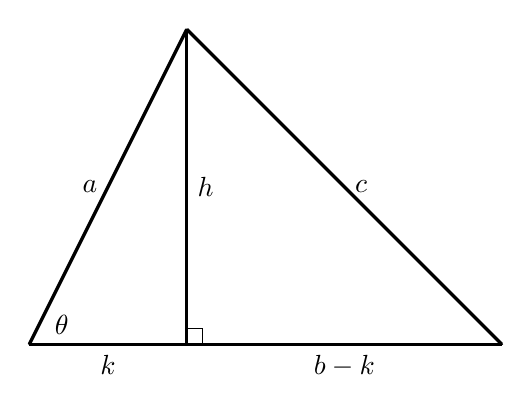
\begin{tikzpicture}[scale=2]
  \draw[](0,0)--(3,0)--(1,2)--cycle;
  \draw[very thick](1,0)--node[below]{$b-k$}(3,0);
  \draw[very thick](1,0)--node[below]{$k$}(0,0);
  \draw[very thick](0,0)--node[left]{$a$}(1,2);
  \draw[very thick](3,0)--node[right]{$c$}(1,2);
  \draw[very thick](1,0)--node[right]{$h$}(1,2);
  \draw[](1.1,0)--(1.1,0.1)--(1,0.1);
  \node[above right] at (0.1,0) {$\theta$};
\end{tikzpicture}\qquad
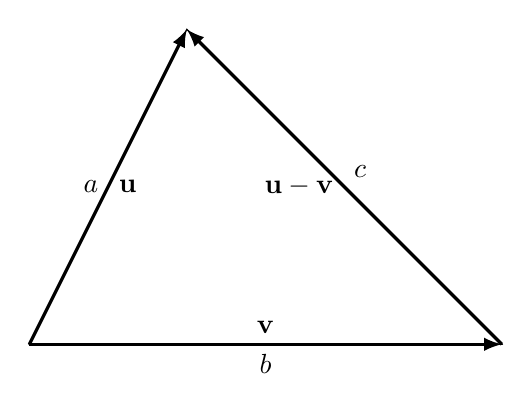
\begin{tikzpicture}[scale=2]
  \draw[](0,0)--(3,0)--(1,2)--cycle;
  \draw[-latex,very thick](0,0)--node[above]{$\vv$}(3,0);
  \draw[-latex,very thick](0,0)--node[right]{$\uu$}(1,2);
  \draw[-latex,very thick](3,0)--node[left]{$\uu-\vv$}(1,2);
  \node[below]at(1.5,0){$b$};
  \node[left]at(0.5,1){$a$};
  \node[above right]at(2,1){$c$};
\end{tikzpicture}
\end{center}
In parts (a)-(g), you will derive the identity $\uu \cdot \vv = \| \uu \| \| \vv \| \cos \theta$.
In parts (h)-(i), you will derive the identity $\| \uu \times \vv \| = \| \uu \| \| \vv \| \sin \theta$.
\begin{enumerate}[label=(\alph*)]
\item Write an identity that relates $a$, $h$, and $k$.
\item Write an identity that relates $c$, $h$, and $b-k$.
\item Write an identity that relates $a$, $k$, and $\theta$.
\item From the three identities above, eliminate the variables $h$ and $k$.  This
  should leave you with the Law of Cosines, $c^2 = a^2 + b^2 - 2 a b \cos
  \theta$.
\item Rewrite the Law of Cosines in terms of the vectors $\uu$, $\vv$, and $\theta$.  $a$, $b$, and $c$ should not appear in your expression.
\item Expand the left hand side.  This should result in a term containing $\uu \cdot \vv$.
\item Solve for $\uu \cdot \vv$ and simplify.
\item Let the components of $\uu$ and $\vv$ be given as $\uu = (u_1, u_2, u_3)$ and $\vv = (v_1, v_2, v_3)$.  Show algebraically, by expanding in terms of the components, that 
  $$
\| \uu \times \vv \|^2 + (\uu \cdot \vv)^2 =    \| \uu \|^2 \| \vv \|^2.
  $$
\item Use the identity from part (h) and the expression derived in part (g) to solve for $\| \uu \times \vv \|$, and simplify.
\end{enumerate}
\end{problem}

\begin{solution}
  \textbf{\textcolor{red}{\TODO}}
\end{solution}

\begin{problem}
Given the triangle with vertices $(0, 2, -1)$, $(2, 0, -1),$ and $(1, 0, 0)$,
calculate the normal of the plane that contains the triangle.
\end{problem}

\begin{solution}
  \textbf{\textcolor{red}{\TODO}}
\end{solution}

\section*{Part 2: Matrices}

\begin{align*}
  \AA &= \mx{1 & 2 & 5 \\ 3 & 7 & 19} &
  \BB &= \mx{5 & 2 \\ 1 & -3 \\ -1 & 1} &
  \uu &= \mx{1\\ 2}
\end{align*}

\begin{problem}
Calculate: (a) $\AA+\BB^T$, (b) $\AA\BB$, and (c) $(\AA\BB)^{-1}$.
\end{problem}

\begin{solution}
  \textbf{\textcolor{red}{\TODO}}
\end{solution}

\begin{problem}
Solve $(\AA\BB)\xx = \uu$ for $\xx$.
\end{problem}

\begin{solution}
  \textbf{\textcolor{red}{\TODO}}
\end{solution}

\begin{problem}
Show that $\AA\BB \ne \BB\AA$.
\end{problem}

\begin{solution}
  \textbf{\textcolor{red}{\TODO}}
\end{solution}

\begin{problem}
  Let $\CC = \mx{c_{11} & c_{12} \\ c_{21} & c_{22}}$, $\DD = \mx{d_{11} &
    d_{12} \\ d_{21} & d_{22}}$, and $\vv = \mx{v_1 \\ v_2}$.  Show that
  $(\CC\DD)\vv = \CC(\DD\vv)$ by calculating $\AA=\CC\DD$, $\ww=\DD\vv$,
  $\AA\vv$, and $\CC\ww$.
\end{problem}

\begin{solution}
  \textbf{\textcolor{red}{\TODO}}
\end{solution}

\end{document}
